%% abtex2-modelo-trabalho-academico.tex, v-1.9.6 laurocesar
%% Copyright 2012-2016 by abnTeX2 group at http://www.abntex.net.br/ 
%%
%% This work may be distributed and/or modified under the
%% conditions of the LaTeX Project Public License, either version 1.3
%% of this license or (at your option) any later version.
%% The latest version of this license is in
%%   http://www.latex-project.org/lppl.txt
%% and version 1.3 or later is part of all distributions of LaTeX
%% version 2005/12/01 or later.
%%
%% This work has the LPPL maintenance status `maintained'.
%% 
%% The Current Maintainer of this work is the abnTeX2 team, led
%% by Lauro César Araujo. Further information are available on 
%% http://www.abntex.net.br/
%%
%% This work consists of the files abntex2-modelo-trabalho-academico.tex,
%% abntex2-modelo-include-comandos and abntex2-modelo-references.bib
%%

% ------------------------------------------------------------------------
% ------------------------------------------------------------------------
% abnTeX2: Modelo de Trabalho Academico (tese de doutorado, dissertacao de
% mestrado e trabalhos monograficos em geral) em conformidade com 
% ABNT NBR 14724:2011: Informacao e documentacao - Trabalhos academicos -
% Apresentacao
% ------------------------------------------------------------------------
% ------------------------------------------------------------------------


\documentclass[
  10.5pt,				  % tamanho da fonte
	openright,			% capítulos começam em pág ímpar (insere página vazia caso preciso)
	twoside,			  % para impressão em recto e verso. Oposto a oneside  
  a5paper,
  chapter=TITLE,	% títulos de capítulos convertidos em letras maiúsculas
	section=TITLE,	% títulos de seções convertidos em letras maiúsculas
  hyphens,        % faz a quebra de linhas em URLs muito longas
	% -- opções do pacote babel --
	english,        % idioma adicional para hifenização
	brazil          % o último idioma é o principal do documento
]{abntex2}

% ---
% Pacotes básicos 
% ---
\usepackage{lmodern}          % Usa a fonte Latin Modern			
\usepackage[T1]{fontenc}      % Selecao de codigos de fonte.
\usepackage[utf8]{inputenc}	  % Codificacao do documento (conversão automática dos acentos)
\usepackage{lastpage}         % Usado pela Ficha catalográfica
\usepackage{indentfirst}      % Indenta o primeiro parágrafo de cada seção.
\usepackage{color}				    % Controle das cores
\usepackage{graphicx}			    % Inclusão de gráficos
\usepackage{microtype} 			  % Para melhorias de justificação
\usepackage[final]{pdfpages}
\usepackage{listings}         % Para incluir código fonte com formatação
\usepackage{lscape}           % Folha em formato landscape

\usepackage{multirow}         % Permite a mesclagem de linhas em tabelas
%\usepackage{adjustbox}        % Permite o escalonamento do conteúdo que não cabe em uma página
%\usepackage{tabularx}         % Impede o overflow de tabelas. 
%\usepackage{rotating}         % Rotaciona tabelas.
%\usepackage{placeins}         % Permite usar \FloatBarrier

% ---

% ---
% Pacotes adicionais, usados apenas no âmbito do Modelo Canônico do abnteX2
% ---
\usepackage{lipsum}				% para geração de dummy text
%\usepackage{cmap}
% ---

% ---
% Lista de símbolos e acrônimos
% ---
%\usepackage{abntex2glossaries}  % Deve ser incluído antes de abntex2cite

% ---
% Pacotes de citações
% ---
\usepackage[brazilian,hyperpageref]{backref} % Paginas com as citações na bibl
\usepackage[alf]{abntex2cite}	               % Citações utilizando o padrão autor-data de chamadas
%\usepackage[num,overcite]{abntex2cite}       % Citações utilizando o padrão numérico de chamadas
\citebrackets()


% --- 
% CONFIGURAÇÕES DE PACOTES
% --- 

% ---
% Configurações do pacote backref
% Usado sem a opção hyperpageref de backref
\renewcommand{\backrefpagesname}{Citado na(s) página(s):~}
% Texto padrão antes do número das páginas
\renewcommand{\backref}{}
% Define os textos da citação
\renewcommand*{\backrefalt}[4]{
	\ifcase #1 %
		Nenhuma citação no texto.%
	\or
		Citado na página #2.%
	\else
		Citado #1 vezes nas páginas #2.%
	\fi}%
% ---

% ---
% Correção das margens
% ---
\setlrmarginsandblock{2.5cm}{1.5cm}{*}
\setulmarginsandblock{2.0cm}{1.5cm}{*}
\checkandfixthelayout
% ---
% Correção das fontes das seções
% ---
%\renewcommand{\ABNTEXchapterfont}{\fontfamily{lm}\fontseries{b}\selectfont}
\renewcommand{\ABNTEXchapterfont}{\fontfamily{cmr}\fontseries{b}\selectfont}
\renewcommand{\ABNTEXchapterfontsize}{\normalsize}
\renewcommand{\ABNTEXsectionfont}{\ABNTEXchapterfont}
\renewcommand{\ABNTEXsectionfontsize}{\normalsize}
\renewcommand{\ABNTEXsubsectionfont}{\ABNTEXchapterfont}
\renewcommand{\ABNTEXsubsectionfontsize}{\normalsize}
\renewcommand{\ABNTEXsubsubsectionfont}{\ABNTEXchapterfont}
\renewcommand{\ABNTEXsubsubsectionfontsize}{\normalsize}
% ---
% Correção do espaçamento no primeiro parágrafo
% ---
\setlength\afterchapskip{\lineskip}
% ---
% Caminho para as imagens
% ---
\graphicspath{{./img/}}
% ---
% Listings
% ---
\renewcommand{\lstlistingname}{Algoritmo}% Listing -> Algoritmo
\renewcommand{\lstlistlistingname}{Lista de \lstlistingname s}% List of Listings -> Lista de Algoritmos
\definecolor{mygreen}{rgb}{0,0.6,0}
\definecolor{mygray}{rgb}{0.5,0.5,0.5}
\definecolor{mymauve}{rgb}{0.58,0,0.82}
\lstset{ %
  backgroundcolor=\color{white},     % choose the background color;
  basicstyle=\footnotesize\ttfamily, % the size of the fonts that are used for the code
  breakatwhitespace=false,           % sets if automatic breaks should only happen at whitespace
  breaklines=true,                 % sets automatic line breaking
  captionpos=t,                    % sets the caption-position to bottom
  commentstyle=\color{mygreen},    % comment style
  deletekeywords={...},            % if you want to delete keywords from the given language
  escapeinside={\%*}{*)},          % if you want to add LaTeX within your code
  extendedchars=true,              % lets you use non-ASCII characters; for 8-bits encodings only, does not work with UTF-8
  frame=single,	                   % adds a frame around the code
  keepspaces=true,                 % keeps spaces in text, useful for keeping indentation of code (possibly needs columns=flexible)
  keywordstyle=\color{blue},       % keyword style
  language=Java,                   % the language of the code
  morekeywords={*,...},            % if you want to add more keywords to the set
  numbers=none,                    % where to put the line-numbers; possible values are (none, left, right)
  numbersep=5pt,                   % how far the line-numbers are from the code
  numberstyle=\tiny\color{mygray}, % the style that is used for the line-numbers
  rulecolor=\color{black},         % if not set, the frame-color may be changed on line-breaks within not-black text (e.g. comments (green here))
  showspaces=false,                % show spaces everywhere adding particular underscores; it overrides 'showstringspaces'
  showstringspaces=false,          % underline spaces within strings only
  showtabs=false,                  % show tabs within strings adding particular underscores
  stepnumber=2,                    % the step between two line-numbers. If it's 1, each line will be numbered
  stringstyle=\color{mymauve},     % string literal style
  tabsize=2,	                     % sets default tabsize to 2 spaces
  title=\lstname,                  % show the filename of files included with \lstinputlisting; also try caption instead of title
  numberbychapter=false            % number lists by chapter or sequentially from the beginning of the document
}

% ----------------------------------------------------------
% PREÂMBULO
% ----------------------------------------------------------

\titulo{Atualização Tecnológica do Formulário de Inscrição do Processo Seletivo da Pós-Graduação da UFSC}
\autor{Makhles Reuter Lange}
\data{\today}
%\instituicao{Universidade Federal de Santa Catarina}
\instituicao{%
  Universidade Federal de Santa Catarina - UFSC
  \par
  Ciência da Computação}
\local{Florianópolis}
\tipotrabalho{Exemplo para referência futura}
\orientador{Andréia Alves dos Santos Schwaab}
\coorientador{Leandro José Komosinski}
\tipotrabalho{Trabalho de Conclusão de Curso}
\preambulo{Relatório Final do Trabalho de Conclusão do Curso do Curso de Ciências da Computação da Universidade Federal de Santa Catarina.}
%TODO
%\preambulo{Trabalho de Conclusão de Curso submetido ao Curso de Ciências da Computação da Universidade Federal de Santa Catarina para a obtenção do grau de Bacharel em Ciências da Computação.}

% ---
% Configurações de aparência do PDF final

% alterando o aspecto da cor azul
\definecolor{blue}{RGB}{41,5,195}

% informações do PDF
\makeatletter
\hypersetup{
     	%pagebackref=true,
		pdftitle={\@title}, 
		pdfauthor={\@author},
    	pdfsubject={\imprimirpreambulo},
	    pdfcreator={TeXmaker},
		pdfkeywords={tcc}{latex}{primefaces}{java}{jsf}{trabalho acadêmico}, 
		colorlinks=true,       		% false: boxed links; true: colored links
    	linkcolor=blue,          	% color of internal links
    	citecolor=blue,        		% color of links to bibliography
    	filecolor=magenta,      		% color of file links
		urlcolor=blue,
		bookmarksdepth=4
}
\makeatother
% --- 

% --- 
% Espaçamentos entre linhas e parágrafos 
% --- 

% O tamanho do parágrafo é dado por:
\setlength{\parindent}{1.0cm}

% Controle do espaçamento entre um parágrafo e outro:
\setlength{\parskip}{0.2cm}  % tente também \onelineskip

\begin{document}

% Seleciona o idioma do documento (conforme pacotes do babel)
\selectlanguage{brazil}

% Retira espaço extra obsoleto entre as frases.
\frenchspacing


% ----------------------------------------------------------
% ELEMENTOS PRÉ-TEXTUAIS
% ----------------------------------------------------------
\pretextual%
% ---
% Capa
% ---
\imprimircapa%
% ---
% Folha de rosto
% (o * indica que haverá a ficha bibliográfica)
% ---
\imprimirfolhaderosto*%
% ---
\clearpage
%\imprimirfichacatalografica%
%\clearpage

% ----------------------------------------------------------
% FOLHA DE APROVAÇÃO
% ----------------------------------------------------------

% Isto é um exemplo de Folha de aprovação, elemento obrigatório da NBR
% 14724/2011 (seção 4.2.1.3). Você pode utilizar este modelo até a aprovação
% do trabalho. Após isso, substitua todo o conteúdo deste arquivo por uma
% imagem da página assinada pela banca com o comando abaixo:
%
%\includepdf{folhadeaprovacaoassinada.pdf}
%
%TODO 
%\begin{folhadeaprovacao}
%
%  \begin{center}
%    {\ABNTEXchapterfont\large\imprimirautor}
%
%    \vspace*{\fill}\vspace*{\fill}
%    \begin{center}
%      \ABNTEXchapterfont\bfseries\Large\imprimirtitulo
%    \end{center}
%    \vspace*{\fill}
%    
%    \hspace{.45\textwidth}
%    \begin{minipage}{.5\textwidth}
%        \imprimirpreambulo
%    \end{minipage}%
%    \vspace*{\fill}
%   \end{center}
%        
%   Trabalho aprovado. \imprimirlocal, \imprimirdata:
%
%   \assinatura{\textbf{\imprimirorientador} \\ Orientador} 
%   \assinatura{\textbf{\imprimircoorientador} \\ Coorientador}
%   \assinatura{\textbf{Beatriz Wilges} \\ Convidado 1}
%   \assinatura{\textbf{Verônica de Souza de Melo} \\ Convidado 2}
%
%   \begin{comment}
%  \begin{center}
%    \vspace*{0.5cm}
%    {\large\imprimirlocal}
%    \par
%    {\large\imprimirdata}
%    \vspace*{1cm}
%  \end{center}
%  \end{comment}
%\end{folhadeaprovacao}


% ----------------------------------------------------------
% RESUMOS
% ----------------------------------------------------------
%TODO 
%\begin{resumo}
%Texto do resumo.
%\vspace{\onelineskip} \\
%\noindent \textbf{Palavras-chave:} Formulário de Inscrição; Processo Seletivo; JavaServer Faces; Primefaces;
%\end{resumo}
%% ---
%\begin{resumo}[Abstract]
%\begin{otherlanguage*}{english}
%The abstract.
%\vspace{\onelineskip} \\
%\noindent \textbf{Keywords:} Application Form; Selective Process; JavaServer Faces; Primefaces;
%\end{otherlanguage*}
%\end{resumo}


% ---
% Lista de ilustrações
% ---
%\pdfbookmark[0]{\listfigurename}{lof}
%\listoffigures*
%\cleardoublepage
% ---

% ---
% Lista de tabelas
% ---
%\pdfbookmark[0]{\listtablename}{lot}
%\listoftables*
%\cleardoublepage
% ---

% ---
% Lista de abreviaturas e siglas
% ---
%TODO
%\begin{siglas}
%  \item[Java EE] Java Enterprise Edition
%  \item[JSF]     JavaServer Faces
%  \item[JPA]     Java Persistence API
%  \item[SeTIC]   Superintendência de Governança Eletrônica e Tecnologia da Informação e Comunicação
%  \item[UFSC]    Universidade Federal de Santa Catarina
%  \item[RUP]     Rational Unified Process
%  \item[UML]     Unified Modelling Language
%\end{siglas}



% ----------------------------------------------------------
% SUMÁRIO
% ----------------------------------------------------------
\pdfbookmark[0]{\contentsname}{toc}
\tableofcontents*
\cleardoublepage
% ---



% ----------------------------------------------------------
% ELEMENTOS TEXTUAIS
% ----------------------------------------------------------
\textual%


\pagenumbering{arabic}
\setcounter{page}{5}

\chapter{Introdução}
% ----------------------------------------------------------

% ---
\section{Contextualização}
% ---

O acesso aos cursos de Pós-Graduação da UFSC é feito através de processos seletivos. Atualmente, existe um sistema\footnote{Vide \href{}{http://www.capg.ufsc.br/inscricao}} com poucas funcionalidades que está sendo utilizado por secretarias de alguns cursos. Outras utilizam o seu próprio formulário de inscrição online, enquanto que algumas não utilizam nenhum sistema de inscrição propriamente dito, restringindo-se ao uso de formulários de inscrição manuais.

O uso desses diversos sistemas de inscrição, com suas funcionalidades e interfaces distintas, acarreta em diversos problemas, tais como:
\begin{itemize}
  \item Falta de padronização dos requisitos e tecnologias utilizadas.
  \item Autenticação de forma não-centralizada, o que além de ser uma vulnerabilidade em termos de segurança, implica em duplicação de código.
  \item Difícil manutenibilidade;
  \item Difícil obtenção de estatísticas relacionadas aos candidatos.
\end{itemize}

Não obstante, o sistema atual está carente de algumas funcionalidades consideradas primordiais, descritas nos itens a seguir. A implementação de tais funcionalidades no sistema atual é custosa, pois sua estrutura contempla os requisitos definidos na época da elaboração do sistema. Adicionalmente, as bibliotecas e tecnologias utilizadas no sistema atual são antigas\footnote{Algumas estão, inclusive, descontinuadas.}, dificultando seu desenvolvimento e sua manutenibilidade. Justifica-se, portanto, a atualização tecnológica do sistema de inscrição.

\subsection{Envio de documentos}
A funcionalidade mais importante que será implementada neste novo sistema é a possibilidade do envio de documentos por parte dos candidatos, que atualmente têm o trabalho de comparecer às secretarias dos cursos com as cópias dos documentos. A praticidade dessa funcionalidade beneficia tanto o candidato quanto a universidade.

\subsection{Salvamento das informações}
Caso um candidato queira fazer a inscrição em algum dos programas disponibilizados pela UFSC através do sistema de inscrição atual, este deve, essencialmente, fornecer todas as informações em uma única sessão e, ao final, receberá um número de inscrição e a possibilidade de imprimir um comprovante de inscrição. Pretende-se oferecer ao candidato a opção de salvar o progresso do preenchimento do formulário. O candidato poderá, dessa forma, distribuir o preenchimento do formulário em várias sessões até que esteja seguro das informações fornecidas e decida-se por finalizar sua inscrição.

\subsection{Ordem de preenchimento do formulário}
No sistema atual, o preenchimento do formulário segue uma ordem predefinida. Muitas vezes, no entanto, o candidato não possui todas as informações necessárias e/ou relevantes ao iniciar o preenchimento do formulário. Pretende-se dar a possibilidade de preenchimento do formulário sem nenhuma ordem imposta neste processo\footnote{A não ser, é claro, em situações onde exista uma ordem implícita. O envio de documentos é um exemplo, pois estes dependem do programa e nível escolhidos.}.

% ---
\section{SeTIC}
% ---

A Superintendência de Governança Eletrônica e Tecnologia da Informação e Comunicação (SeTIC), setor de informática da Universidade Federal de Santa Catarina (UFSC), é responsável pelo planejamento, pesquisa, aplicação e desenvolvimento de produtos e serviços de tecnologia da informação e comunicação da universidade\footnote{Mais informações em http://setic.ufsc.br/apresentacao/}.

Ressalta-se que o autor deste trabalho já foi estagiário na SeTIC e atualmente possui bolsa de extensão pela FEESC. Todas as atividades estão sendo desenvolvidas nas instalações da SeTIC, com equipamentos e tecnologias disponibilizados por esta. Assim, o último estágio do desenvolvimento do presente sistema, \emph{i.e.}, a \emph{operação} e a \emph{manutenção}\footnote{O sistema é liberado e implantado no ambiente de produção. Eventuais erros que não foram descobertos nos estágios anteriores e novos requisitos podem surgir ao longo do uso do sistema, justificando a sua constante manutenção.}, serão feitas pela SeTIC.

% ---
\section{Objetivos}
% ---

% ---
\subsection{Objetivo Geral}
% ---
O objetivo principal deste Trabalho de Conclusão de Curso é desenvolver um sistema para a inscrição de candidatos nos processos seletivos dos diversos programas de Pós-Graduação da UFSC, utilizando o sistema de inscrição que está em uso atualmente como base.

% ---
\subsection{Objetivos Específicos}
% ---
\begin{itemize}
  \item Implementar o Módulo de Inscrição - consiste na implementação das regras de negócio e das páginas que o candidato terá acesso ao realizar sua inscrição.
  \item Implementar o Módulo Administrativo - consiste na implementação das regras de negócio no sistema CAPG Secretaria (sistema em desenvolvimento para administração dos cursos por suas secretarias).
  \item Elaborar um artigo referente ao TCC.
\end{itemize}

% ---
\section{Resultados Esperados}
% ---
\begin{itemize}
  \item Módulo do Formulário de Inscrição.
  \item Módulo Administrativo do Processo de Inscrição.
  \item Artigo referente à produção realizada anexo ao TCC.
\end{itemize}



\chapter{Fundamentação Teórica}
% ----------------------------------------------------------

% ---
\section{Aplicações Web}
% ---


% ---
\section{Plataforma Java, Edição Empresarial}\label{sec:java2e}
% ---

As \textbf{aplicações empresariais} têm o propósito de fornecer a \emph{lógica do negócio} de uma empresa. O seu gerenciamento é feito de forma centralizada e é comum a sua interação com outros softwares empresariais. A plataforma Java, Edição Empresarial (Java EE), é um conjunto de tecnologias Java que são utilizadas para o desenvolvimento de aplicações empresariais. O objetivo da plataforma é fornecer aos desenvolvedores um conjunto de especificações / APIs que permitam a diminuição do tempo de desenvolvimento, a redução da complexidade e o aumento do desempenho de aplicações empresariais \cite{javaee7}. Tais especificações são \emph{contratos} que são implementados por diversos fornecedores, \emph{e.g.}, GlassFish, Oracle WebLogic, Apache TomEE, etc.

% ---
\subsection{Aplicações Multi-Camadas}
% ---

Segundo o modelo Java EE, as aplicações são distribuídas em camadas (\emph{tiered design})\footnote{Os termos \emph{tier} e \emph{layer} são ambos traduzidos para o português como ``camada''. No entanto, uma \emph{tier} representa uma unidade física, na qual um código ou processo é executado. Uma \emph{layer}, por sua vez, representa uma unidade lógica, responsável pela organização lógica do código através da abstração dos dados. Diversas \emph{layers} podem existir em computadores diferentes, ou em processos diferentes em um único computador, ou ainda em um único processo em um único computador \cite{lhotka}.}. Define-se, desta forma, responsabilidades distintas para as diferentes partes do sistema, \emph{i.e.}, para os diferentes componentes que compõem uma aplicação Java EE (vide Figura~\ref{fig:multitiered_app}) e que são distribuídos nas camadas Cliente, Web, Negócio e EIS.

\begin{figure}[!ht]
  \caption{\label{fig:multitiered_app}Componentes Java EE distribuídos nas diversas camadas de duas aplicações Web.}
  \begin{center}
    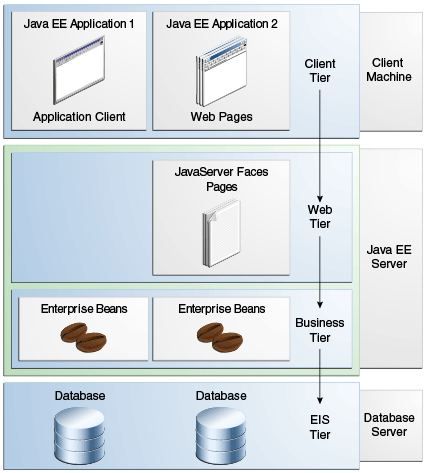
\includegraphics[width=0.75\textwidth]{multitiered_applications.png}
  \end{center}
  \fonte{adaptado de \citetext{javaee7}}
\end{figure}

% ---
\subsubsection{Camada Cliente}
% ---

Esta camada é composta de clientes aplicativos que acessam o servidor Java EE e que geralmente se localizam em máquinas diferentes da máquina do servidor:

\begin{itemize}
  \item Clientes Web - também chamados de \emph{clientes magros}, são compostos de páginas dinâmicas (\emph{e.g.}, XHTML) geradas na camada Web e por um navegador responsável por renderizá-las.
  \item Clientes Aplicativos - quando os usuários necessitam realizar atividades que requerem uma interface mais rica do que a disponibilizada por linguagens de marcação, utilizam-se clientes aplicativos baseados nas APIs Swing ou AWT (\emph{Abstract Window Toolkit})\footnote{Não obstante, pode-se utilizar uma interface em linha de comando.}. Embora seja possível o estabelecimento de uma conexão HTTP com um \emph{servlet} na camada Web, clientes aplicativos costumam acessar diretamente os \emph{beans} gerenciais da camada de negócio.
  \item \emph{Applets} - componentes embarcados que são incluídos nas páginas web. São escritos em Java e, portanto, necessitam da máquina virtual Java instalada no navegador web do cliente (e provavelmente do \emph{plugin} Java e de um arquivo de política de segurança).
\end{itemize}

% ---
\subsubsection{Camada Web}\label{sec:camada-web}
% ---

É a camada responsável pela interação entre os clientes e a camada de negócios. Suas principais funções são:
\begin{itemize}
  \item Gerar, dinamicamente, conteúdo para o cliente em diversos formatos.
  \item Obter as entradas (dados e ações) da interface com o cliente e retornar os resultados dos componentes da camada de negócios.
  \item Controlar o fluxo das páginas no cliente.
  \item Manter o estado dos dados da sessão do usuário.
  \item Executar um pouco de lógica simples e armazenar dados em componentes JavaBeans temporariamente.
\end{itemize}

\emph{Servlets} e páginas web criadas com a tecnologia \emph{JavaServer Faces} (vide seção~\ref{sec:jsf}) são os componentes desta camada. \emph{Servlets} são classes Java que possuem métodos adequados a receber requisições e construir respostas às tais requisições dinamicamente. O trecho de código a seguir (vide Algoritmo~\ref{alg:servlet}) representa um \texttt{HttpServlet} que atende a requisições HTTP do tipo GET através da sobrescrita do método \texttt{doGet()}. Os parâmetros \texttt{HttpServletRequest} e \texttt{HttpServletResponse} representam, respectivamente, a requisição feita pelo cliente e a resposta do servidor.
%
\begin{lstlisting}[language=Java, caption={Um \emph{servlet} que imprime ``\emph{Hello World}''.}, label={alg:servlet}]
import java.io.*;
import javax.servlet.*;
import javax.servlet.http.*;

public class HelloWorld extends HttpServlet {
  public void doGet(HttpServletRequest req,
                    HttpServletResponse res)
      throws ServletException, IOException {
    res.setContentType("text/html");
    PrintWriter out = res.getWriter();
    out.println("<html>");
    out.println("<head><title>Hello World</title></head>");
    out.println("<body>");
    out.println("<big>Hello World</big>");
    out.println("</body></html>");
  }
}
\end{lstlisting}
\fonte{adaptado de \citeonline{javaservlet}}

Um \emph{servlet} HTTP pode, além do método \texttt{doGet()}, sobreescrever outros métodos, tais como \texttt{doPut()}, \texttt{doDelete()}, etc, que representam requisições HTTP do tipo PUT, DELETE, etc, respectivamente.


% ---
\subsubsection{Camada de Negócio}\label{sec:camada-negocio}
% ---
A camada de negócios possui componentes que provêm a lógica do negócio da aplicação, ou seja, código que provê funcionalidades para um determinado domínio do negócio. As tecnologias utilizadas nessa camada são as seguintes:
\begin{itemize}
  \item Componentes Enterprise JavaBeans (EJB), que fornecem funcionalidades como gerenciamento de sessão, segurança, gerenciamento de transações, etc.
  \item \emph{Web services} (JAX-RS, JAX-WS).
  \item Entidades de persistência - Java Persistence API (JPA).
\end{itemize}


% ---
\subsubsection{Camada EIS}
% ---

A camada EIS consiste de servidores de bancos de dados, sistemas de planejamento de recursos empresariais e outras fontes de dados legados. Esses recursos geralmente se localizam em suas próprias máquinas e são acessados pela camada de negócios. As tecnologias utilizadas nessa camada são:
\begin{itemize}
  \item Java Database Connetivity API (JDBC) - uma interface que permite a conexão às bases de dados.
  \item Java Persistence API (JPA).
  \item Java Transaction API (JTA) - uma interface para a realização de transações.
\end{itemize}

% ---
\subsection{JavaServer Faces}\label{sec:jsf}
% ---

A tecnologia JavaServer Faces (JSF) é uma \emph{especificação} de uma API Java utilizada para a criação de interfaces de usuário em aplicações web. Com essa API, é possível:
%
\begin{itemize}
  \item Representar componentes\footnote{Componentes, ou \emph{widgets}, são entidades autônomas e reutilizáveis da interface de usuário.} e o gerenciamento dos seus estados;
  \item Fazer o controle de eventos;
  \item Realizar a validação e a conversão de dados no lado do servidor;
  \item Definir regras para a navegação entre páginas;
  \item Prover o suporte à internacionalização e acessibilidade;
\end{itemize}
%

Existem duas implementações principais: Apache MyFaces e Oracle Mojarra. Ambas contêm pelo menos os componentes padrões, ou seja, os componentes responsáveis por gerar qualquer um dos elementos HTML básicos (tabelas, caixas de entrada de texto, botões, seletores, etc). 


\subsubsection{Arquitetura do \emph{Framework}}

O \emph{framework} JSF segue o padrão arquitetural\footnote{Um padrão arquitetural expressa um esquema de organização estrutural para sistemas baseados em \emph{software}. O padrão provê um conjunto de subsistemas predefinidos, especifica suas responsabilidades, e inclui regras e diretrizes para organizar a relação entre eles \cite{buschmann96}.} MVC baseado em componentes. A grande vantagem do padrão MVC é a separação entre apresentação e comportamento (lógica) da aplicação:

\begin{description}
  \item[Visão] - fornece a representação da informação para o usuário da aplicação. Pode-se ter diversas visões do mesmo modelo. A tecnologia padrão utilizada pelo JSF é a Facelets (vide Seção~\ref{sec:facelets}).
  \item[Modelo] - representa o comportamento da aplicação em termos do domínio do problema, e independe da visão.
  \item[Controlador] - converte entradas/eventos em comandos para a visão ou para o modelo.
\end{description}

Todas as requisições feitas à aplicação devem passar primeiramente pelo controlador através do \texttt{FacesServlet}, que é o \emph{servlet} responsável por gerenciar o ciclo de vida do processamento de requisições. Ou seja, o próprio \emph{framework} JSF assume o papel de controlador no padrão MVC (vide esquema A na Figura~\ref{fig:mvc}). Dessa forma, o desenvolvedor da aplicação não precisa se preocupar em escrever código \emph{boilerplate} tal como o do Algoritmo~\ref{alg:servlet}.
A implementação de controladores para atender a diferentes tipos de requisições, tais como o mostrado no Algoritmo~\ref{alg:servlet}, é utilizada em \emph{action-based frameworks} (SpringMVC, Struts, ASP.NET, etc).

A Figura~\ref{fig:mvc} mostra esquemas representativos destes dois modelos MVC. Em (A), tem-se o \emph{framework} JSF, baseado em componentes. Resumidamente, a requisição feita pelo usuário da aplicação é recebida pelo \texttt{FacesServlet}, que delega o processamento para a visão responsável pela geração da página acessada. O componente acessado (por exemplo, um botão) invoca um método em um \emph{managed bean}\footnote{Uma classe Java que trabalha junto à visão.}. Este, por sua vez, pode buscar dados do modelo e retorná-los para a visão. Finalmente, a visão envia a resposta ao usuário. O ciclo de vida do processamento de requisições do JSF é bem mais complexo, pois envolve a criação de uma árvore de componentes, a conversão e validação dos dados obtidos destes componentes, o gerenciamento de eventos oriundos destes componentes e a propagação dos dados para os \emph{beans}.

\begin{figure}[!ht]
  \caption{\label{fig:mvc}Comparação entre os dois tipos de padrão MVC. Em (A), tem-se o \emph{framework} baseado em componentes. Em (B), o baseado em ações. Os números ao lado das setas indicam a ordem do processamento de uma requisição.}
  \begin{center}
    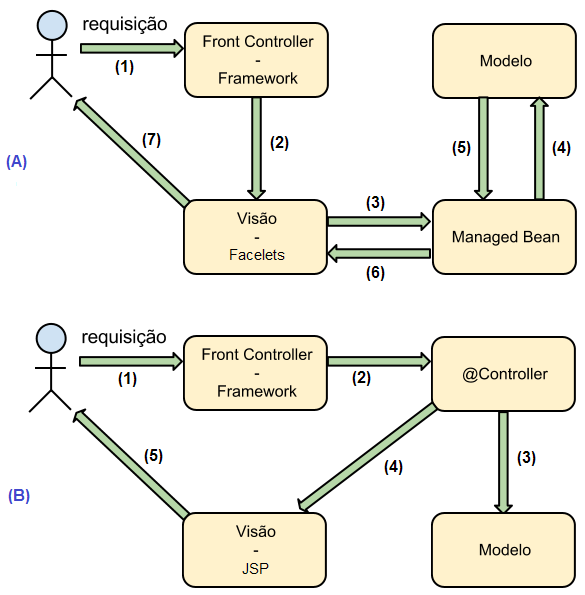
\includegraphics[width=0.75\textwidth]{/mvc/mvc.png}
  \end{center}
  \fonte{Caelum. Adaptado de \citetext{caelum}}
\end{figure}

No esquema (B), o desenvolvedor da aplicação deve criar classes controladoras\footnote{Classes que estendem a classe \texttt{HttpServlet}.} para tratar as diversas requisições, invocando o modelo e atualizando a visão. 



% ---
\subsection{Facelets}\label{sec:facelets}
% ---
\emph{Facelets} é uma tecnologia de apresentação utilizada em aplicações baseadas em JSF. Atualmente, é também a tecnologia definida na especificação do JSF, substituindo assim a descontinuada JSP (JavaServer Pages).

Com esta tecnologia, as páginas web são criadas em XHTML e os componentes são inseridos através de \emph{tags} de diversas bibliotecas. No Algoritmo~\ref{alg:tags}, por exemplo, utiliza-se as \emph{tags} \texttt{<h:inputText>} e \texttt{<f:validateLongRange>}, das bibliotecas  JSF HTML e Core, respectivamente, para a entrada de texto e validação desse texto (após sua conversão) entre um valor mínimo e um valor máximo.

\begin{lstlisting}[language=html, caption={Utilização de \emph{tags} em um arquivo XHTML.}, label={alg:tags}]
<html xmlns="http://www.w3.org/1999/xhtml"
      xmlns:h="http://xmlns.jcp.org/jsf/html"
      xmlns:f="http://xmlns.jcp.org/jsf/core">

<h:body>
  <h:form>
    <h:inputText id="userNumber"
                 title="Insira um numero entre 0 e 10:"
                 value="#{aBean.userNumber}">
      <f:validateLongRange minimum="#{aBean.minimum}"
                           maximum="#{aBean.maximum}"/>
    </h:inputText>
    <h:commandButton id="submit"
                     value="Submit"
                     action="response"/>
  </h:form>
</h:body>
\end{lstlisting}
\fonte{Adaptado de \citeonline{javaee7}.}


Dentre suas vantagens, \cite{javaee7} destacam:
\begin{itemize}
  \item Reuso de código através de \emph{templates} e da composição de componentes.
  \item Redução do tempo de compilação.
  \item Validação de expressões em \emph{Expression Language} em tempo de compilação.
\end{itemize}


% ---
\subsection{Primefaces}
% ---
Bibliotecas de componentes oferecem funcionalidades previamente  testadas e eventualmente úteis, tais como tabelas capazes de ordenar, filtrar e selecionar linhas, organização do conteúdo em diversos tipos de painéis e menus, exibição de coleções em listas e árvores, etc, além da possibilidade de escolha de diversos temas. Existem diversas bibliotecas disponíveis. As mais conhecidas são: PrimeFaces, RichFaces e ICEFaces. Nos sistemas atualmente desenvolvidos pela SeTIC baseados em Java, utiliza-se a biblioteca PrimeFaces. A Figura~\ref{fig:primefaces_datatable} mostra um exemplo de tabela feita com essa biblioteca.

\begin{figure}[!ht]
  \caption{\label{fig:primefaces_datatable}Componente DataTable da biblioteca PrimeFaces. Evidencia-se o uso de um \emph{paginator} no topo da tabela e o uso do tema \emph{bluesky}.}
  \begin{center}
    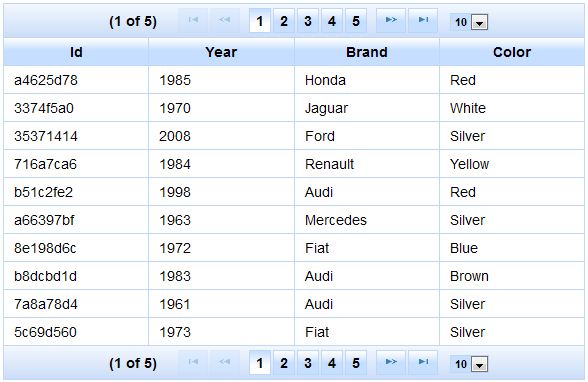
\includegraphics[width=0.75\textwidth]{/primefaces/datatable.png}
  \end{center}
  \fonte{PrimeFaces. Disponível em \url{https://www.primefaces.org/showcase/}}
\end{figure}

% ---
\subsection{Java Persistence API}
% ---

A API de Persistência do Java (JPA - Java Persistence API), possibilita o gerenciamento de dados relacionais nas aplicações Java através de um mapeamento objeto-relacional. Esse mapeamento é feito através de \emph{entidades} - objetos do domínio de persistência. Uma entidade representa uma tabela de um banco de dados no modelo relacional, e suas instâncias representam as linhas desta tabela. Segundo \citeonline{javaee7}, para ser considerada uma entidade, uma classe precisa:

\begin{enumerate}
  \item Possuir a anotação \texttt{javax.persistence.entity};
  \item Pelo menos um construtor sem argumentos com visibilidade \emph{public} ou \emph{protected};
  \item A classe, suas instâncias persistíveis e seus métodos não podem ser declarados \emph{final};
  \item Instâncias persistíveis devem ser declaradas como \emph{private}, \emph{protected} ou \emph{package private} e podem ser acessadas somente através dos métodos da classe.
\end{enumerate}

O estado de uma entidade é definido através de seus campos persistíveis, os quais usam anotações de mapeamento objeto-relacional para mapear as entidades e seus relacionamentos aos dados da base de dados. As restrições impostas anteriormente e o relacionamento entre campos podem ser vistos na entidade \texttt{PoloCursoNivel} do Algoritmo~\ref{alg:entity_pcn}, no qual as restrições foram destacadas com comentários.

Pode-se perceber o relacionamento entre as entidades PoloCursoNivel e Polo através das anotações \texttt{@ManyToOne} e \texttt{@JoinColumn}. Neste caso, várias instâncias de \texttt{PoloCursoNivel} podem referenciar a mesma instância de \texttt{Polo}. No banco de dados, a tabela \texttt{poloCursoNivel\_cnp} (mapeada através da anotação \texttt{@table}) contém a coluna \texttt{cd\_polo\_pol} (indicada pelo parâmetro \texttt{name}), que é uma chave estrangeira para a coluna de mesmo nome na tabela mapeada da entidade \texttt{Polo} (anotada na classe \texttt{Polo} e, portanto, não mostrada na imagem).

\begin{lstlisting}[caption={Entidade PoloCursoNivel e seus mapeamentos.}, label={alg:entity_pcn}]

@Entity // 1)
@Table(name="poloCursoNivel_cnp", catalog = "capg",
       schema = "dbo")
public class PoloCursoNivel implements Serializable {

    private static final long serialVersionUID = 1L;

    @Id
    private PoloCursoNivelPK id;

    @ManyToOne
    @JoinColumn(name="cd_polo_pol",
                referencedColumnName="cd_polo_pol")
    private Polo polo;  // 3 e 4)

    @ManyToOne
    @JoinColumns({
        @JoinColumn(name = "cd_curso_cur",
                    referencedColumnName = "cd_curso_cur"),
        @JoinColumn(name = "cd_nivel_niv",
                    referencedColumnName = "cd_nivel_niv")
    })
    private Curso curso;

    // Demais campos

    public PoloCursoNivel() {  // 2)
        super();
    }

    // Getters e setters
}

\end{lstlisting}
\fonte{Adaptado de \citeonline{keith2013}.}


\citeonline{keith2013} definem outras anotações utilizadas no relacionamento de entidades além de \texttt{@ManyToOne}. As principais e/ou mais utilizadas são discutidas brevemente nos itens a seguir.

\subsubsection{Relacionamento \texttt{@OneToOne}}
Apenas uma instância da entidade fonte\footnote{A entidade na qual se está fazendo a anotação.} pode referenciar a mesma instância da entidade alvo. Em termos do banco de dados, isso implica na existência de uma restrição de unicidade na coluna da chave estrangeira da tabela fonte. Ainda, o JPA espera que o nome dessa coluna seja igual ao nome do atributo da entidade fonte seguido de um \emph{underscore} e do nome da coluna da chave primária da tabela alvo. Caso esse não seja o caso, então deve-se fornecer o nome da coluna na anotação \texttt{@JoinColumn}.

Para ilustrar essa situação, considere as tabelas ilustradas na Figura~\ref{fig:jpa_onetoone}. O mapeamento feito pelo JPA espera que a coluna com a chave estrangeira a ser utilizada seja chamada de \texttt{PARKINGSPACE\_ID}, porém essa coluna chama-se \texttt{PSPACE\_ID}. Neste caso, utiliza-se a anotação \texttt{@JoinColumn(name = ``PSPACE\_ID'')}, conforme Algoritmo~\ref{alg:entity_employee}.



\begin{figure}[!ht]
  \caption{\label{fig:jpa_onetoone} Tabelas EMPLOYEE e PARKING\_SPACE.}
  \begin{center}
    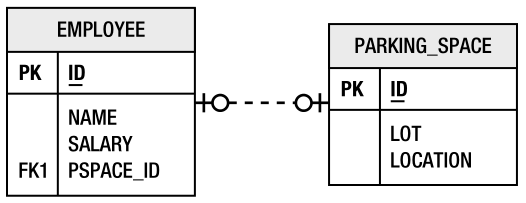
\includegraphics[width=0.75\textwidth]{/jpa/one_to_one_table.png}
  \end{center}
  \fonte{Retirado de \citeonline{keith2013}.}
\end{figure}

É interessante notar que o campo \texttt{name} não possui nenhuma anotação relacionada à sua persistência. Isso se deve ao fato de existir uma coluna de mesmo nome na tabela \texttt{EMPLOYEE}.

\begin{lstlisting}[caption={Classe Employee e seus relacionamentos.}, label={alg:entity_employee}]
@Entity
public class Employee {

  @Id private long id;
  
  @OneToOne
  @JoinColumn(name = "PSPACE_ID")
  private ParkingSpace parkingSpace;
  // ...
}
\end{lstlisting}
\fonte{Adaptado de \citeonline{keith2013}.}


Quando a entidade alvo do relacionamento também possuir uma referência à entidade fonte, tem-se então um relacionamento bidirecional, em que uma das entidades é dita ser a \emph{dona} do relacionamento por conter a coluna com a chave estrangeira da outra entidade\footnote{A escolha de qual das tabelas deverá conter a chave estrangeira da outra tabela é uma decisão de modelagem do banco de dados.}. Nessa situação, a anotação \texttt{@JoinColumn} da entidade que \emph{não} é a dona do relacionamento recebe o elemento \texttt{mappedBy = "X"}, onde X refere-se ao nome do campo da entidade que é dona do relacionamento, como pode ser visto no Algoritmo~\ref{alg:entity_employee_bi}.

\begin{lstlisting}[caption={Classe ParkingSpace e seus relacionamentos.}, label={alg:entity_employee_bi}]
@Entity
public class ParkingSpace {
  
  @Id private long id;
  private String location;

  @OneToOne(mappedBy = "parkingSpace")
  private Employee employee;
  // ...
}
\end{lstlisting}
\fonte{Adaptado de \citeonline{keith2013}.}%

\subsubsection{Relacionamento \texttt{@OneToMany}}

Este tipo de relacionamento ocorre quando uma entidade está associada a uma coleção de entidades. Considere as tabelas \texttt{EMPLOYEE} e \texttt{DEPARTMENT} ilustradas na Figura~\ref{fig:jpa_onetomany}. O relacionamento \emph{um para muitos} feito em UML pode ser visto em (b).

\begin{figure}[!ht]
  \caption{\label{fig:jpa_onetomany} Tabelas \texttt{EMPLOYEE} e \texttt{DEPARTMENT} em (a) e seu relacionamento em (b).}
  \begin{center}
    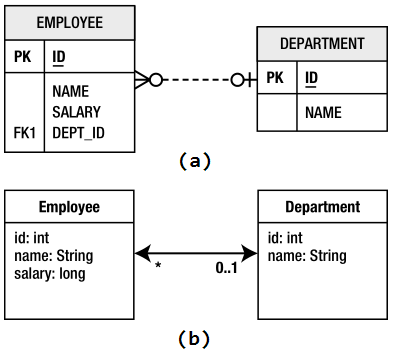
\includegraphics[width=0.75\textwidth]{/jpa/one_to_many.png}
  \end{center}
  \fonte{Adaptado de \citeonline{keith2013}.}
\end{figure}


É importante notar que esse relacionamento implica em um relacionamento \emph{muitos para um} quando analisado a partir da tabela \texttt{EMPLOYEE} e, portanto, é um relacionamento naturalmente bidirecional. Daí que uma das entidades fará o papel de dona do relacionamento, conforme discutido anteriormente no caso do relacionamento \emph{um para um} bidirecional. Devido ao fato de não existir uma maneira escalonável de guardar inúmeras chaves em uma única linha de uma tabela, a entidade dona do relacionamento nessa situação deve ser a que estiver no lado ``muitos''. Nesse caso, a entidade dona é, portanto, a \texttt{EMPLOYEE} e nela estarão as chaves estrangeiras para as linhas da tabela \texttt{DEPARTMENT}. Por sua vez, isso implica na adição do elemento \texttt{mappedBy} na anotação \texttt{@JoinColumn} dessa última entidade, conforme Algoritmo~\ref{alg:entity_dept}.

\begin{lstlisting}[caption={Classe Department e seus relacionamentos.}, label={alg:entity_dept}]
@Entity
  public class Department {

  @Id
  private long id;
  private String name;

  @OneToMany(mappedBy = "department")
  private Collection<Employee> employees;
  // ...
}
\end{lstlisting}
\fonte{Adaptado de \citeonline{keith2013}.}%

Mais uma vez, devido à utilização de um nome de coluna diferente do valor padrão esperado para esse relacionamento, utiliza-se o elemento \texttt{name} na anotação \texttt{@JoinColumn} da entidade Employee (vide Algoritmo~\ref{alg:entity_employee2}).

\begin{lstlisting}[caption={Classe Employee e seus relacionamentos.}, label={alg:entity_employee2}]
@Entity
public class Employee {

  @Id
  private long id;

  @ManyToOne
  @JoinColumn(name = "DEPT_ID")
  private Department department;
  // ...
}
\end{lstlisting}
\fonte{Adaptado de \citeonline{keith2013}.}%


\subsubsection{Relacionamento \texttt{@ManyToMany}}

O último tipo de relacionamento entre entidades apresentado é chamado de \emph{muitos para muitos}. Esse relacionamento ocorre quando uma ou mais entidades fonte estão associadas a uma coleção de entidades alvo, e estas entidades alvo estão associadas a uma coleção de entidades fonte. A representação dessa situação em UML pode ser vista no item (b) da Figura~\ref{fig:jpa_manytomany} para as entidades Employee e Project.

Considere agora as tabelas ilustradas no item (a) da Figura~\ref{fig:jpa_manytomany}. Uma linha de \texttt{EMPLOYEE} pode estar associada a diversas linhas de \texttt{PROJECT} e vice-versa. A existência da tabela \texttt{EMP\_PROJ} justifica-se por não ser escalável guardar as chaves estrangeiras em cada linha de \emph{ambas} as tabelas. Nesse caso, \texttt{EMP\_PROJ} possui apenas duas colunas e estas guardam as chaves estrangeiras de cada uma das tabelas. Portanto, \texttt{EMPLOYEE} não possui uma coluna com as chaves estrageiras de \texttt{PROJECT} e vice-versa \cite{keith2013}.

\begin{figure}[!ht]
  \caption{\label{fig:jpa_manytomany} Tabelas \texttt{EMPLOYEE},  \texttt{EMP\_PROJ} e \texttt{PROJECT} em (a) e seu relacionamento em (b).}
  \begin{center}
    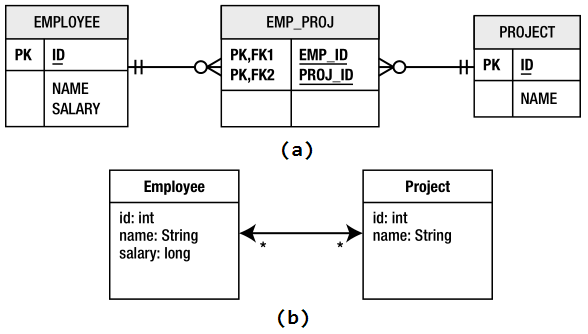
\includegraphics[width=1.0\textwidth]{/jpa/many_to_many.png}
  \end{center}
  \fonte{Adaptado de \citeonline{keith2013}.}
\end{figure}

Se ambas as tabelas \texttt{EMPLOYEE} e \texttt{PROJECT} não possuem uma coluna de chaves estrangeiras, quem é a entidade dona do relacionamento? A resposta é: tanto faz, desde que essa decisão seja indicada ao JPA. As entidades Employee e Project resultantes do mapeamento podem ser vistas no Algoritmo~\ref{alg:entity_employee_project}. Evidencia-se o uso da anotação \texttt{joinColumns}, indicando a entidade dona do relacionamento.


\begin{lstlisting}[caption={Classes Employee e Project.}, label={alg:entity_employee_project}]
@Entity
public class Employee {
  @Id
  private long id;
  private String name;
  @ManyToMany
  @JoinTable(name="EMP_PROJ",
      joinColumns=@JoinColumn(name="EMP_ID"),
      inverseJoinColumns=@JoinColumn(name="PROJ_ID"))
  private Collection<Project> projects;
  // ...
}

@Entity
public class Project {
  @Id
  private long id;
  private String name;
  @ManyToMany(mappedBy="projects")
  private Collection<Employee> employees;
  // ...
}
\end{lstlisting}
\fonte{Adaptado de \citeonline{keith2013}.}%

% ---
%\subsection{Hibernate}
% ---

% ---
%\subsection{Spring}
% ---



\chapter{Análise e Projeto - Módulo de Inscrição}
% ----------------------------------------------------------

\citeonline{sommerville2011} explica que um \emph{processo de software} é um conjunto de atividades relacionadas que levam à produção de um produto de software. Embora existam diversos processos de software, todos devem incluir as seguintes atividades fundamentais: especificação, projeto e implementação, validação, e evolução do software. Cada uma destas atividades é uma tarefa complexa em si mesma e inclui subatividades.

Por não existir um modelo de processo de software único a ser utilizado na SeTIC, o autor decidiu-se por utilizar o mesmo ``modelo'' de processo de software dos projetos anteriores em que participou na SeTIC como estagiário: as atividades fundamentais supracitadas são executadas de forma iterativa, seguindo as boas práticas especificadas pelo \emph{Rational Unified Process} (RUP), um modelo de processo moderno e híbrido, derivado de trabalhos sobre a UML (Unified Modelling Language).

Ressalta-se que o desenvolvimento se dá por meio da extensão e melhoria de um sistema existente. Far-se-á uso das tabelas utilizadas nesse sistema, bem como dos campos presentes no formulário de inscrição. Não obstante, novas tabelas e campos serão criados, e a implementação das regras de negócio será realizada pelo autor deste trabalho.


% ---
\section{Elicitação, Análise e Definição de Requisitos}
% ---

O desenvolvimento de um software/sistema segundo o modelo adotado pode ser dividido em diversos estágios. O primeiro consiste na elicitação, análise e definição de requisitos. Segundo \citeonline{sommerville2011}, os requisitos de um sistema são as descrições do que o sistema deve fazer, os serviços que oferece e as restrições a seu funcionamento. Esses requisitos refletem as necessidaeds dos clientes para um sistema que serve a uma finalidade determinada, como controlar um dispositivo, fazer um pedido ou encontrar informações. Esta etapa é muito importante pois, além de servir de base para as demais etapas, fornece um rumo a ser seguido e um objetivo a ser alcançado. Não menos importante, evita a implementação de funcionalidades desnecessárias.

A elicitação ou descoberta dos requisitos do sistema pode ser feita de diversas maneiras: entrevistas, cenários, casos de uso, etnografia, etc. A abordagem adotada aqui, comum aos demais sistemas desenvolvidos na SeTIC, foi a de realização de entrevistas abertas, isto é, uma série de questões relacionadas ao uso do sistema foi explorada junto ao cliente. Dessa forma, pôde-se obter uma melhor compreensão de suas necessidades.

Até o momento da confecção deste relatório, duas reuniões foram realizadas com o cliente. Um conjunto de \emph{wireframes} das páginas do sistema foi desenvolvido\footnote{Utilizou-se um \emph{plugin} do WireframeSketcher feito para o Eclipse.} e apresentado com o objetivo de validar a estrutura, o conteúdo, as diversas funções e os diversos caminhos de interações dos usuários com o sistema. A confecção deste conjunto de \emph{wireframes} teve como base o sistema atual. Em cima deste foram aplicadas todas as mudanças que se faziam necessárias e que justificam o desenvolvimento do novo sistema. A Figura~\ref{fig:wireframe} fornece um exemplo retirado deste conjunto: após ter feito \emph{login} no sistema, o usuário Fulano é recebido com um conjunto de inscrições previamente realizadas por si. Evidencia-se o uso de balões explicativos para agilizar o entendimento dos diversos elementos da página pelo cliente. Ressalta-se que o visual da página não é o foco do \emph{wireframe}, e sim o que ela permite que o usuário realize.

\begin{figure}[!ht]
  \caption{\label{fig:wireframe} \emph{Wireframe} que representa a página de inscrições realizadas pelo usuário Fulano após este ter feito \emph{login} no sistema. }
  \begin{center}
    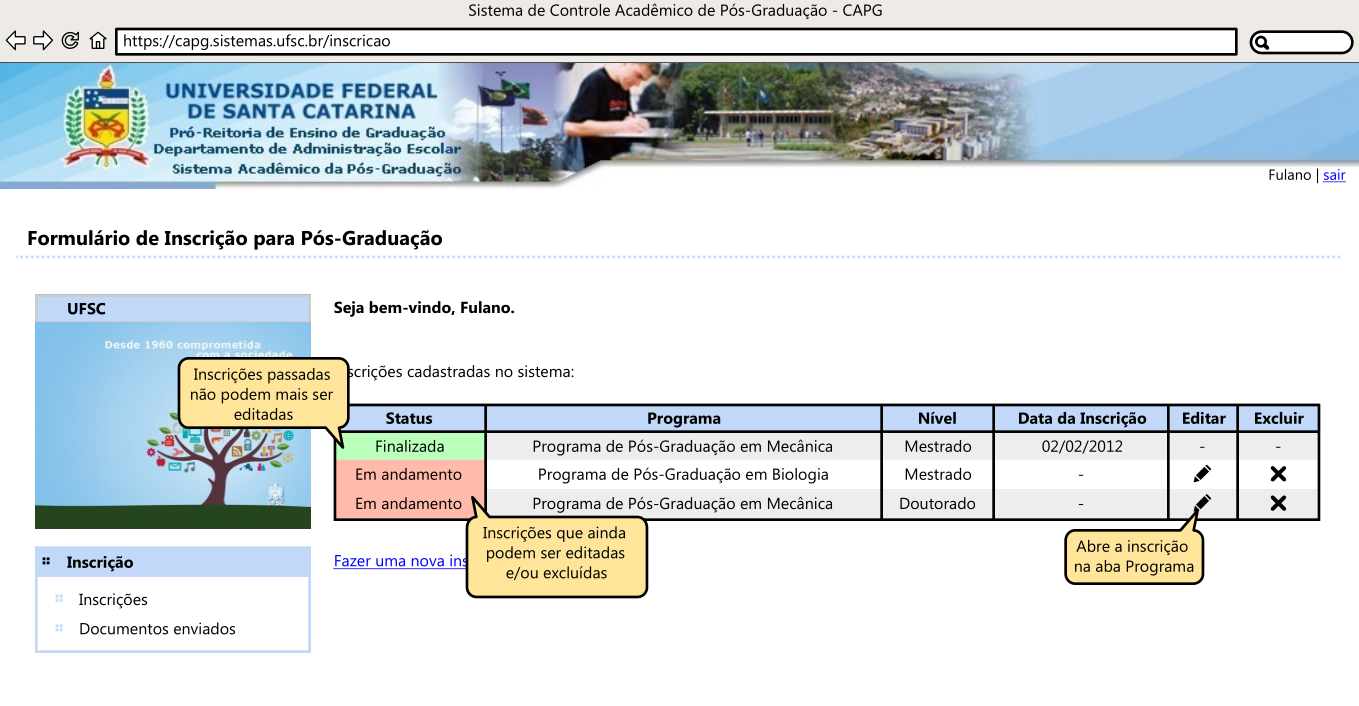
\includegraphics[width=1.0\textwidth]{/wireframe.png}
  \end{center}
  \fonte{Produzido pelo autor.}
\end{figure}

Na reunião com o cliente, os requisitos propostos e exemplificados nos \emph{wireframes} foram analisados. Destes, alguns foram removidos, outros adicionados. No fim, um conjunto de requisitos iniciais\footnote{Em princípio, segundo o modelo em cascata, cada estágio só se inicia após o término do anterior. Na prática, há uma sobreposição dos estágios: problemas com os requisitos são identificados durante o projeto e erros de programa aparecem durante a fase de operação e manutenção, exigindo uma reavaliação dos requisitos.} para o sistema foi aprovado e servirá como uma especificação formal para o desenvolvimento do sistema. Embora a distinção entre os diferentes tipos de requisitos não seja tão clara, os requisitos de software são frequentemente classificados como \emph{funcionais} e \emph{não funcionais}. Essa classificação é abordada nos itens a seguir.

\subsection{Requisitos Funcionais}\label{sec:requisitos_funcionais}

Os requisitos funcionais descrevem os serviços que o sistema deve fornecer, como deve reagir a entradas específicas e como deve se comportar em determinadas situações. A sua descrição é feita aqui de forma abstrata (em alto nível) para que sejam compreendidos pelos diversos \emph{stakeholders} do projeto.

\begin{description}
\item[Requisito 1 - Visualizar programas oferecidos.] O usuário poderá visualizar a lista de programas de pós-graduação oferecidos pela UFSC sem a necessidade de realizar \emph{login} no sistema.
\item[Requisito 2 - Realizar cadastro no CAS.] O usuário poderá se cadastrar no Sistema de Autenticação Centralizada a partir da página inicial do sistema.
\item[Requisito 3 - Acessar o sistema.] O usuário poderá acessar o sistema através de \emph{login}.
\item[Requisito 4 - Sair do sistema.] O usuário poderá sair do sistema a qualquer momento fazendo \emph{logout}.
\item[Requisito 5 - Salvar a inscrição.] O usuário poderá salvar as informações inseridas no formulário para um acesso futuro.
\item[Requisito 6 - Alterar informações.] O usuário poderá alterar as informações inseridas durante todo o período de inscrição do programa selecionado, desde que não tenha finalizado a sua inscrição.
\item[Requisito 7 - Finalizar a inscrição.] O usuário poderá finalizar a sua inscrição. Após finalizada, o usuário receberá um número de inscrição e os dados inseridos não poderão mais ser modificados.
\item[Requisito 8 - Imprimir um comprovante de inscrição.] Após finalizada a inscrição, o usuário poderá imprimir um comprovante de inscrição.
\item[Requisito 9 - Importar dados do CAS.] O usuário poderá importar os dados que foram utilizados para fazer o cadastro no CAS.
\item[Requisito 10 - Importar dados de inscrições anteriores.] O usuário poderá importar alguns dados de inscrições anteriores ao iniciar uma nova inscrição. Os dados que poderão ser importados serão definidos pela PROPG.
\item[Requisito 11 - Fazer \emph{upload} de arquivos.] O usuário poderá fazer o \emph{upload} de arquivos solicitados pelo programa escolhido.
\item[Requisito 12 - Importar arquivos.] O usuário poderá importar arquivos utilizados em inscrições anteriores.
\item[Requisito 13 - Visualizar inscrição.] O usuário poderá visualizar os dados de sua inscrição em uma página única antes de decidir-se por finalizar a inscrição.
\item[Requisito 14 - Inserir informações.] O usuário poderá inserir diversos tipos de informações, as quais são agrupadas em dados do programa, pessoais, econômicos, de contato e de formação. Embora esses dados não estejam descritos em pormenores neste relatório, estavam presentes nos protótipos apresentados à PROPG na reunião de definição dos requisitos.
\end{description}


\subsection{Requisitos Não Funcionais}

Segundo \citeonline{sommerville2011}, os requisitos não funcionais são aqueles que não estão diretamente relacionados com os serviços específicos oferecidos pelo sistema a seus usuários. Relacionam-se às propriedades emergentes do sistema e definem restrições sobre a sua implementação. Foram identificados os seguintes requisitos:

\begin{itemize}
\item O sistema deve possibilitar o acesso dos usuários durante todos os dias do ano para que possam imprimir comprovantes de inscrição.
\item Usuários do sistema devem autenticar-se utilizando o Sistema de Autenticação Centralizada (CAS).
\item A aplicação Web deve ser feita utilizando a linguagem de programação Java e as tecnologias que são comumente utilizadas no desenvolvimento Web com Java e que estão disponíveis na SeTIC (vide Seção~\ref{sec:java2e}).
\item A aplicação Web deve utilizar a estrutura e seguir o visual dos demais sistemas desenvolvidos na SeTIC. Para tanto, deve-se utilizar o projeto denominado \emph{Projeto Base}, criado por desenvolvedores da SeTIC para o desenvolvimento de novos sistemas.
\end{itemize}

% ---
\section{Projeto do Sistema}
% ---

O segundo estágio do modelo de desenvolvimento de software adotado consiste em desenvolver a arquitetura geral do sistema. Aqui descrevem-se as principais abstrações do sistema e seus relacionamentos através dos diagramas de casos de uso e de classes.

\subsection{Diagrama de Casos de Uso}

Diagramas de casos de uso fornecem uma representação em alto nível da interação entre os diversos usuários (chamados de atores) com o sistema. As interações são representadas por elipses e os atores por bonecos palito. A Figura~\ref{fig:use_cases} abaixo relaciona os casos de uso identificados para o ator Candidato, único ator do módulo de inscrição.

\begin{figure}[!ht]
  \caption{\label{fig:use_cases} Casos de uso identificados para o ator Candidato. }
  \begin{center}
    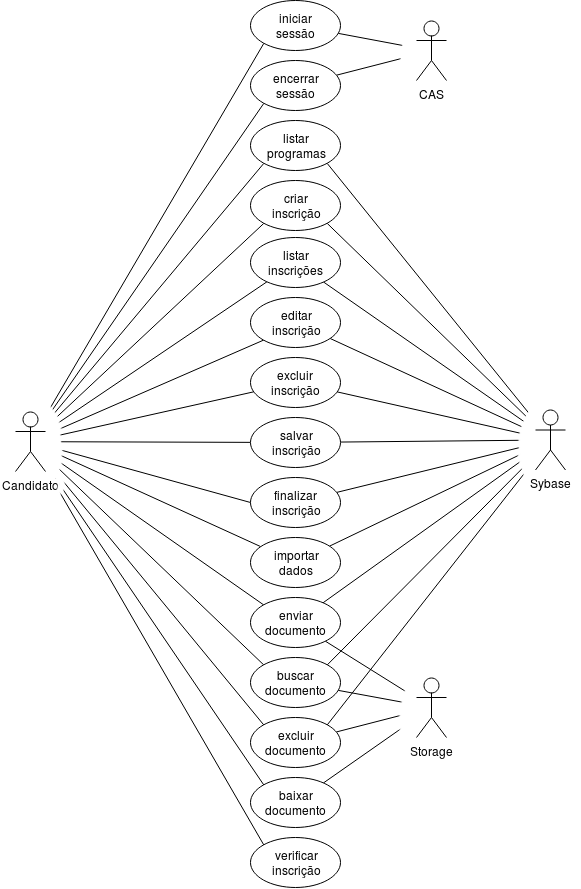
\includegraphics[width=0.8\textwidth]{/use_cases.png}
  \end{center}
  \fonte{Elaborada pelo autor.}%
\end{figure}

% ---
\subsection{Diagrama de Classes}
% ---

Um diagrama de classes é responsável por mostrar as diversas classes de uma aplicação e as associações (agregação, composição, generalização e dependências) entre elas.

O diagrama de classes do sistema foi dividido em duas imagens por questão de espaço. A Figura~\ref{fig:uml_classes1} mostra as classes envolvidas na obtenção dos programas disponíveis em uma determinada data. Pode-se perceber uma associação de generalização entre as classes \texttt{ProgramasService} e \texttt{ProgramasServiceImpl} e dependências entre as classes \texttt{ProgramasBean} e \texttt{ProgramaAux}, e \texttt{ProgramasBean} e \texttt{ProgramasService}.

\begin{figure}[!ht]
  \caption{\label{fig:uml_classes1} Modelo entidade-relacionamento relacionado à obtenção de programas. }
  \begin{center}
    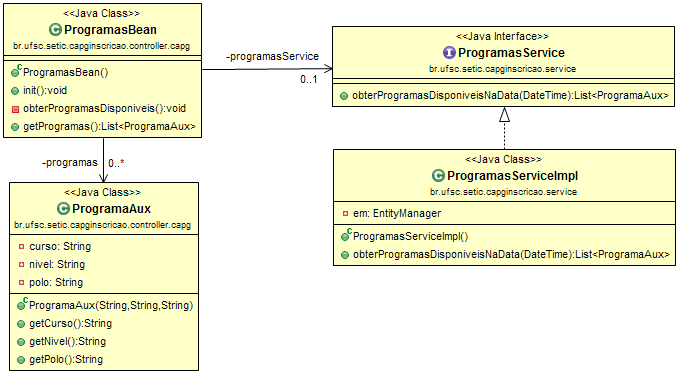
\includegraphics[width=1.0\textwidth]{/uml/programas.png}
  \end{center}
  \fonte{Elaborada pelo autor com a ferramenta ObjectAid UML Explorer.}%
\end{figure}

A Figura~\ref{fig:uml_classes2} ilustra a classe \texttt{InscricoesBean} e algumas das suas associações de dependência. As dependências dessas classes não são mostradas (este diagrama pode crescer substancialmente). As classes \texttt{Curso} e \texttt{Nivel} são entidades e estão relacionadas entre si. \texttt{InscricoesService} é uma interface que provê serviços à classe \texttt{InscricoesBean} (através de uma classe que a implemente). Finalmente, \texttt{InscricaoAux} é uma classe auxiliar que é utilizada junto à \emph{view} para exibir informações das inscrições cadastradas para um determinado usuário.

\begin{landscape}
\begin{figure}[!ht]
  \caption{\label{fig:uml_classes2} Modelo entidade-relacionamento relacionado às inscrições. }
  \begin{center}
    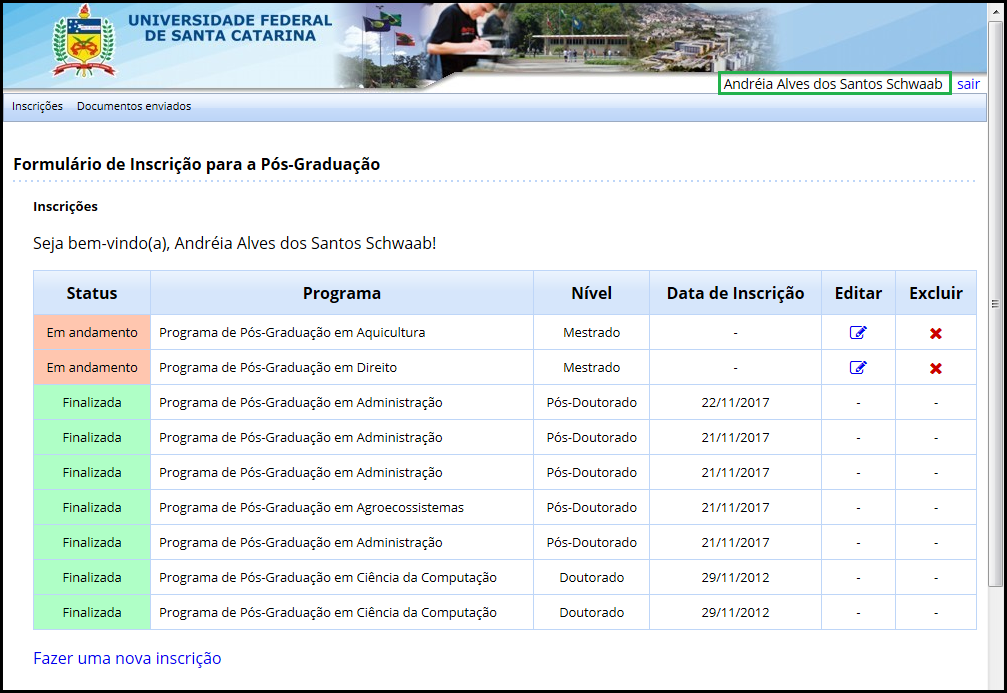
\includegraphics[scale=0.40]{/uml/inscricoes.png}
  \end{center}
  \fonte{Elaborada pelo autor com a ferramenta ObjectAid UML Explorer.}%
\end{figure}
\end{landscape}


% ---
\section{Implementação}
% ---

Após definida a estrutura inicial do sistema, deu-se início ao processo de implementação. O projeto foi configurado para atender às necessidades do sistema. Além de arquivos de configuração, diversos pacotes foram criados para a separação lógica das classes, como pode ser visto na Figura~\ref{fig:src_explorer}.

\begin{figure}[!ht]
  \caption{\label{fig:src_explorer} Alguns pacotes e classes da aplicação vistos no Eclipse. }
  \begin{center}
    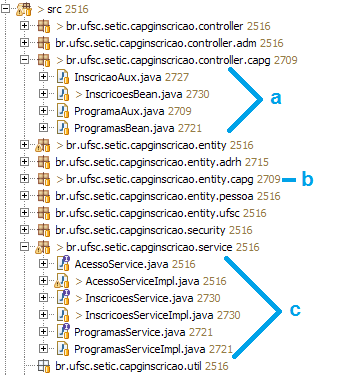
\includegraphics[scale=0.85]{/src_explorer.png}
  \end{center}
  \fonte{Elaborada pelo autor.}
\end{figure}

O pacote \texttt{(a)} é composto de \emph{beans} e classes auxialiares da camada Web (vide Seção~\ref{sec:camada-web}) que, em conjunto com os arquivos .xhtml, são responsáveis por gerar as páginas da aplicação.

O mapeamento objeto-relacional se encontra no pacote destacado por \texttt{(b)}. Aqui se encontram as classes das inúmeras entidades do sistema (vide Seção~\ref{sec:camada-negocio}) e, por serem muitas, não foram incluídas na imagem.

As classes representadas por \texttt{(c)}, assim como as classes do item anterior, pertencem à camada de negócios. São classes ditas de serviço, responsáveis pelas operações básicas de persistência: \emph{Create}, \emph{Read}, \emph{Update}, \emph{Delete}, comumente abreaviadas por CRUD. Na imagem, as classes \texttt{AcessoService}, \texttt{InscricoesService} e \texttt{InscricoesService} são interfaces\footnote{Em Java, uma interface é um tipo abstrato que especifica um comportamento que deve ser implementado.}, enquanto que \texttt{AcessoServiceImpl}, \texttt{InscricoesServiceImpl} e \texttt{InscricoesServiceImpl} representam suas implementações.



Para ilustrar a operação \emph{read}, o Algoritmo~\ref{alg:programas_disponiveis} contém o método que obtém a lista de programas disponíveis em uma determinada data. Percebe-se que o tipo do elemento contido na lista é um \texttt{ProgramaAux}, uma das classes auxialiares mencionadas no item \texttt{(a)}. Ainda, \texttt{em} é uma instância de um \texttt{EntityManager} que está associada a um contexto de persistência.
%TODO - referenciar JPA

Ressalta-se que a maioria das classes presentes na Figura~\ref{fig:src_explorer} já existiam no Projeto Base e provêm funcionalidades como segurança (através do Spring), acesso a Web Services, comunição com a base de dados Centura, validadores e conversores do JSF, etc.

\begin{landscape}
\begin{lstlisting}[language=java, caption={Obtenção da lista de programas disponíveis.}, label={alg:programas_disponiveis}]
public List<ProgramaAux> obterProgramasDisponiveisNaData(DateTime data) {
    StringBuffer query = new StringBuffer();
    query.append("SELECT new br.ufsc.setic.capginscricao.controller.capg.ProgramaAux(");
    query.append("ps.curso.nome, ps.nivel.descricao, ps.polo.nome) ");
    query.append("FROM ProcessoSeletivo ps ");
    query.append("WHERE :data BETWEEN ps.dtInicioProcesso AND ps.dtTerminoProcesso ");
    query.append("ORDER BY ps.curso");

    return em.createQuery(query.toString(), ProgramaAux.class)
            .setParameter("data", data.toLocalDateTime())
            .getResultList();
}
\end{lstlisting}
\fonte{Produzido pelo autor.}%
\end{landscape}



% ---
\subsection{Funcionalidades}\label{sec:funcionalidades}
% ---

A Tabela~\ref{tabela-casos-uso} lista os casos de uso relativos aos requisitos especificados na Seção \ref{sec:requisitos_funcionais} e que haviam sido implementados \emph{parcialmente} no momento da confecção deste relatório.


\begin{table}[!htb]
  \IBGEtab{%
    \caption{Casos de uso implementados e respectivas páginas envolvidas.}%
    \label{tabela-casos-uso}
  }{
    \begin{tabular}{|c|c|}
      \hline 
      Caso de Uso & Página da Aplicação \\ \hline 
      Visualizar programas disponíveis & programas.xhtml \\ \hline 
      Fazer \emph{login} & \multirow{2}{*}{login.xhtml} \\
      Fazer \emph{logout} & \\ \hline
      Criar inscrição & \multirow{3}{*}{inscricoes.xhtml} \\
      Editar inscrição & \\
      Excluir inscrição & \\ \hline 
    \end{tabular} 
  }{
    \fonte{Elaborada pelo autor.}%
    %\nota{Esta é uma nota, que diz que os dados são baseados na regressão linear.}%
    %\nota[Anotações]{Uma anotação adicional, seguida de várias outras.}%
  }
\end{table}

Faz-se necessário justificar o uso do termo ``parcialmente'' no parágrafo anterior. Embora a criação e a edição de inscrições tenham sido implementadas, diversas variáveis de controle e mesmo de estado serão criadas ao longo do desenvolvimento deste projeto para atender aos demais requisitos especificados. Muitas dessas variáveis serão utilizadas na criação e edição de inscrições, implicando em uma constante refatoração do código já implementado. Daí que não se pode afirmar que os casos de uso citados tenham sido implementados em sua totalidade.




\chapter{Conclusões}
% ----------------------------------------------------------

O sistema de inscrição atual é utilizado por apenas alguns dos cursos de Pós-Graduação da UFSC. Alguns cursos utilizam seus próprios sistemas, dificultando a sua mantenibilidade e introduzindo duplicações de código e vulnerabilidades.

Torna-se imprescindível, portanto, o desenvolvimento de um novo sistema de inscrição unificado, que dê suporte a novas funcionalidades e que utilize as tecnologias atualmente em uso na SeTIC.

Algumas atividades previstas na proposta do TCC foram desenvolvidas neste primeiro semestre da disciplina de Projetos, especificamente:
\begin{itemize}
  \item Levantamento das funcionalidades;
  \item Especificação dos requisitos do sistema a partir destas funcionalidades
  \item Definição da arquitetura do sistema;
  \item Adequação do Projeto Base para atender a estrutura definida;
  \item implementação dos casos de uso discutidos na Seção~\ref{sec:funcionalidades}.
\end{itemize}



% ----------------------------------------------------------
\bibliography{referencias}

%\begin{thebibliography}{9}
%
%\bibitem{lamport94}
%  Leslie Lamport,
%  \emph{\LaTeX: a document preparation system},
%  Addison Wesley, Massachusetts,
%  2nd edition,
%  1994.
%\end{thebibliography}


\end{document}

% EXEMPLO DE TABELA DO IBGE
%
%\begin{table}[!htb]
%  \IBGEtab{%
%    \caption{Um Exemplo de tabela alinhada que pode ser longa ou curta, conforme padrão IBGE.}%
%    \label{tabela-ibge}
%  }{%
%    \begin{tabular}{ccc}
%      \toprule
%      Nome & Nascimento & Documento \\
%      \midrule \midrule
%      Maria da Silva & 11/11/1111 & 111.111.111-11 \\
%      \bottomrule
%    \end{tabular}%
%  }{%
%    \fonte{Produzido pelos autores}%
%    \nota{Esta é uma nota, que diz que os dados são baseados na regressão linear.}%
%    \nota[Anotações]{Uma anotação adicional, seguida de várias outras.}%
%  }
%\end{table}